\documentclass[main.tex]{subfiles}

\begin{document}
\chapter{Контрольная работа №~1}

Цель работы: Получение базовых знаний и умений в области программирования микроконтроллеров AVR на языке ассемблер.

Работа выполняется в среде Atmel Studio.

\section{Теоретические сведения}

\subsection{Порты ввода/вывода}

Микроконтроллеры AVR имеют в своём составе от одного до семи портов ввода/вывода. Каждый разряд такого порта подсоединён к одному из выводов (контакту/пину) микросхемы. Порты ввода/вывода служат для обмена информацией с внешними устройствами. Каждый порт имеет имя: от \texttt{A} до \texttt{G}.

Для управления каждым портом ввода/вывода используется три так называемых регистра ввода/вывода (далее~--- РВВ). Назначения каждого их этих регистров:

\begin{itemize}
\item \texttt{PORTx}~--- регистр данных, используется для вывода информации;
\item \texttt{DDRx}~--- регистр направления передачи информации (0~--- вход, 1~--- выход);
\item \texttt{PINx}~---регистр ввода информации.
\end{itemize}
где \texttt{x}~--- имя порта.

Например, для порта \texttt{B} существуют следующие регистры: \texttt{PORTB}, \texttt{DDRB} и \texttt{PINB}. 

Отдельные разряды регистров (бит) имеют свои имена. Например, разряды регистра \texttt{PORTB} именуются так: \texttt{PB0}, \texttt{PB1} ... \texttt{PB7}. Имена доступных регистров и их разрядов можно посмотреть в заголовочных (\texttt{.inc}) файлах конкретного микроконтроллера.

Упрощенная функциональная схема одного разряда порта ввода/вывода приведена на рисунке \ref{fig:port1}.

\begin{figure}[t]
\centering
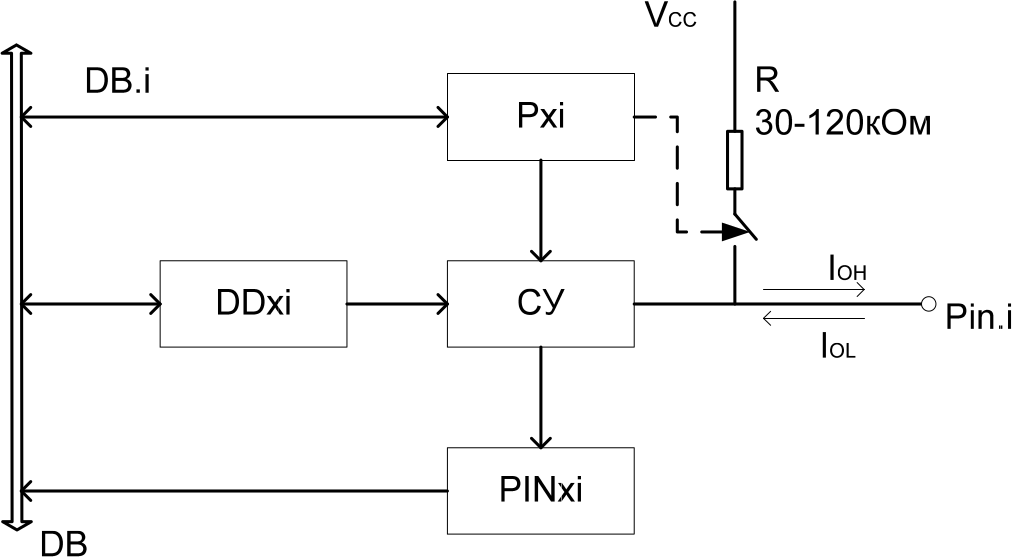
\includegraphics[scale=0.25]{images/port1.png}
\caption{Упрощенная функциональная схема порта ввода/вывода}
\label{fig:port1}
\end{figure}

Каждый разряд порта ввода/вывода  может работать независимо от других разрядов как на ввод, так и на вывод информации. Для переключения режимов работы служит регистр \texttt{DDRx}. Если в разряд этого регистра записана единица, то соответствующий разряд порта работает как выход. Пример: 

\begin{lstlisting}
.include "8515def.inc"  $\color{red}\textrm{; AT90S8515}$
.def tmp = r16          $\color{red}\textrm{; псевдоним для регистра}$

.cseg
reset:
    ldi tmp, 0b11111111 $\color{red}\textrm{; загрузить константу в регистр}$
    out DDRA, tmp       $\color{red}\textrm{; все пины на вывод}$
    ldi tmp, 0b01010101
    out PORTA, tmp      $\color{red}\textrm{; выводим}$
loop:
    rjmp loop
\end{lstlisting}

На рисунке \ref{fig:port2} приведена  более детализированная функциональная схема одного разряда порта, поясняющая основные режимы портов ввода/вывода.


\begin{figure}[t]
\centering
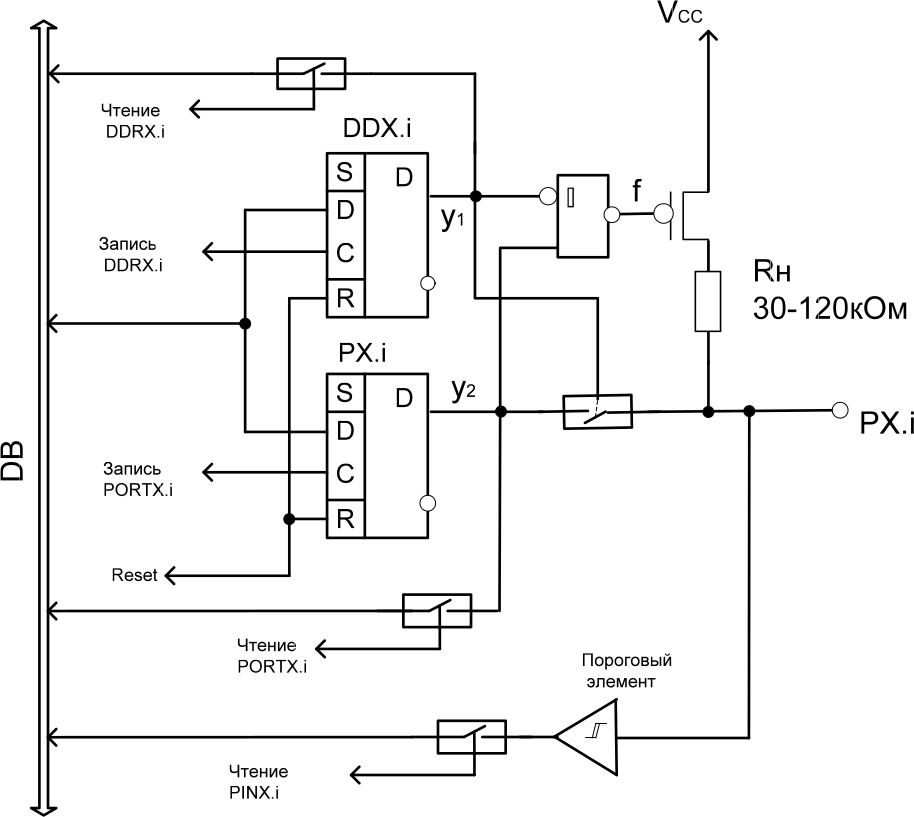
\includegraphics[scale=0.30]{images/port2.png}
\caption{Детализированная функциональная схема порта ввода/вывода}
\label{fig:port2}
\end{figure}







\newpage
\subsection{Прерывания}

В программах, где предполагается использование прерываний, необходимо в начале программируемой памяти микроконтроллера разместить таблицу векторов прерываний, которая содержит команды безусловного перехода \texttt{rjmp} на подпрограммы прерываний~--- обработчики прерываний. Обработчик прерываний должен завершаться командой \texttt{reti}, которая восстанавливает глобальный флаг разрешения прерываний и возвращает управление в место программы, которое выполнялось до срабатывания прерывания.

Общая структура программы с прерываниями:

\begin{lstlisting}
.include "8515def.inc"

.cseg
$\color{red}\textrm{; таблица векторов прерываний}$
.org 0x0000        $\color{red}\textrm{; вектор прерывания}$
    rjmp reset
.org INT0addr      $\color{red}\textrm{; 0x0001}$
    rjmp int0      $\color{red}\textrm{; переход на обработчик прерывания}$

reset:
    $\color{red}\textrm{; ...}$
    sei    $\color{red}\textrm{; установить флаг глобального прерывания}$
loop:
    rjmp loop
        
int0:      $\color{red}\textrm{; обработчик прерывания}$
    $\color{red}\textrm{; ...}$
    reti   $\color{red}\textrm{; выход из обработчика}$
\end{lstlisting}








\newpage
\section{Варианты заданий}\label{ch:var1}

\begin{figure}[h]
\centering
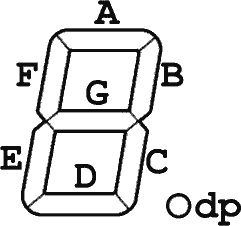
\includegraphics[scale=0.3]{images/pin.png}
\caption{Семисегментный светодиодный индикатор}
\label{fig:pin}
\end{figure}

Задание на контрольную работу: необходимо организовать устройство для отображения информации на семисегментном светодиодном индикаторе. Информация на индикаторе меняется от нажатия клавиш.

При выполнении контрольной работы, обратите внимание на раздел <<\nameref{ch:str}>> (стр.~\pageref{ch:str}).

\begin{small}

\vspace{12px}
\noindent
\begin{tabularx}{\textwidth}{|X|}
\hline
\textbf{Вариант 1}\\
\hline
При включении на индикаторе горит светодиод D.

После каждого размыкания кнопки SA1 циклически загораются горизонтальные светодиоды в восходящем порядке (D-G-A-D-...).

Каждое замыкание кнопки SA2 приводит к изменению порядка загорания светодиодов по размыканиям кнопки SA1.\\
\hline
\end{tabularx}

\vspace{6px}
\noindent
\begin{tabularx}{\textwidth}{|X|}
\hline
\textbf{Вариант 2}\\
\hline
При включении на индикаторе горит светодиод G.

При каждом замыкании кнопки SА1 горящий светодиод перемещается циклически против часовой стрелки по периметру верх­него квадрата (G-B-A-F-G-...), а при каждом замыкании кнопки SA2~--- по часовой стрелке по периметру нижнего квадрата (G-C-D-E-G-...).

При этом если горит какой-либо диод из верхнего квадрата, кроме G, то кнопка SA2 должна быть заблокирована, а если горит диод из нижнего квадрата, кроме G, то блокируется кнопка SA1.\\
\hline
\end{tabularx}

\vspace{6px}
\noindent 
\begin{tabularx}{\textwidth}{|X|}
\hline
\textbf{Вариант 3}\\
\hline
При включении на индикатор выводится «0».

При каждом размыкании кнопки SA1 цифра на индикаторе увеличивается на «1». После достижения «9» счёт начинается с «0». При замыкании кнопки SA2 индикатор гаснет, и дальнейшие нажатия кнопки SA1 игнорируются. При повторном замыкании кнопки SA2 на индикаторе загорается погашенная цифра, и воз­обновляется нормальная работа кнопки SA1.\\
\hline
\end{tabularx}

\vspace{6px}
\noindent 
\begin{tabularx}{\textwidth}{|X|}
\hline
\textbf{Вариант 4}\\
\hline
При включении на индикатор выводится «9».

Первоначально нажатия кнопки SA2 не влияют на содержимое индикатора.

При однократном замыкании кнопки SA1 цифра уменьшается на «1», и разрешается нажатие кнопки SA2 для очередного уменьше­ния цифры на «1», а кнопка SA1 блокируется.

Таким образом, роли кнопок каждый раз меняются местами. После достижения «0» счёт начинается с «9».\\
\hline
\end{tabularx}

\vspace{6px}
\noindent 
\begin{tabularx}{\textwidth}{|X|}
\hline
\textbf{Вариант 5}\\
\hline
При включении индикатор не горит.

При нажатой кнопке SA1 на индикаторе горит верхний квадрат (светодиоды A, B, F, G). При нажатой кнопке SA2~--- нижний квад­рат (светодиоды C, D, E, G). При нажатых обеих кнопках горит цифра <<5>>. При отпущенных кнопках индикатор не горит.\\
\hline
\end{tabularx}

\vspace{6px}
\noindent 
\begin{tabularx}{\textwidth}{|X|}
\hline
\textbf{Вариант 6}\\
\hline
При включении на индикаторе горят светодиоды E и F.

При каждом замыкании кнопки SA2 попеременно загораются вертикальные линии E, F и B, C.

При нажатой кнопке SA1 индикатор гаснет, при отпускании кнопки вновь загорается пара погашенных диодов.\\
\hline
\end{tabularx}

\newpage

\vspace{6px}
\noindent 
\begin{tabularx}{\textwidth}{|X|}
\hline
\textbf{Вариант 7}\\
\hline
При включении на индикаторе горит светодиод А.

При каждом замыкании кнопки SA1 горящий светодиод перемещается циклически по часовой стрелке по периметру индикатора (А-В-С-D-E-F-А-...), а при каждом размыкании кнопки SA2 горя­щий светодиод перемещается циклически против часовой стрелки от текущего положения.\\
\hline
\end{tabularx}

\vspace{6px}
\noindent 
\begin{tabularx}{\textwidth}{|X|}
\hline
\textbf{Вариант 8}\\
\hline
При включении индикатор не горит.

Первоначально при нажатии кнопки SA1 загорается цифра «1». При следующем нажатии кнопки SА1 загорается цифра «3» и так далее.

При нажатии кнопки SА2 загорается цифра «2», при последующем нажатии загорается цифра «4» и так далее.

Если в начале нажималась кнопка SА1, потом SА2, то значение цифры SА1 запоминается. При последующем нажатии SА1 пере­ключение продолжается с запомненной цифры.\\
\hline
\end{tabularx}

\vspace{6px}
\noindent 
\begin{tabularx}{\textwidth}{|X|}
\hline
\textbf{Вариант 9}\\
\hline
При включении на индикаторе горит цифра «3».

При нажатии на кнопку SА1 происходит прибавление 2.

При нажатии на кнопку SА2 происходит вычитание 1.\\
\hline
\end{tabularx}

\vspace{6px}
\noindent 
\begin{tabularx}{\textwidth}{|X|}
\hline
\textbf{Вариант 10}\\
\hline
При включении на индикаторе горит светодиод С.

При нажатии кнопки SА1, загораются два светодиода по пери­метру (В, А), а предыдущий/последний (С) выключается, и так да­лее.

При нажатии кнопки SА2 загораются светодиоды по тому же принципу в обратной последовательности.\\
\hline
\end{tabularx}


\newpage


\vspace{6px}
\noindent 
\begin{tabularx}{\textwidth}{|X|}
\hline
\textbf{Вариант 11}\\
\hline
При включении на индикаторе горят светодиоды D, Е, F.

При нажатии кнопки SА1, загораются светодиоды А, В, С, а све­тодиоды D, Е, F выключаются. При повторном нажатии всё воз­вращается в первоначальное состояние.

При нажатии на кнопку SА2 происходит выключение индикатора. При следующем нажатии происходит включение индикатора с отображением предыдущего состояния.\\
\hline
\end{tabularx}

\vspace{6px}
\noindent 
\begin{tabularx}{\textwidth}{|X|}
\hline
\textbf{Вариант 12}\\
\hline
При включении индикатор не горит.

При нажатии на кнопку SА1, загорается цифра «1». Кнопка SА2 заблокирована. При каждом нажатии на кнопку SА1 к значению прибавляется единица. При достижении цифры «5», кнопка SА1 блокируется, а SА2~--- разблокируется.

При нажатии на кнопку SА2 прибавляется по 2. При достижении «1» кнопка SА2 блокируется, SА1~--- разблокируется.\\
\hline
\end{tabularx}

\vspace{6px}
\noindent 
\begin{tabularx}{\textwidth}{|X|}
\hline
\textbf{Вариант 13}\\
\hline
При включении индикатор не горит.

При нажатии на кнопку SА1 загорается цифра «1», отзеркаленная по вертикали. При повторном нажатии на кнопку SА1 к данному числу прибавляется единица.

При нажатии на кнопку SА2, цифры отображаются правильно. При повторном нажатии на кнопку SА2, к цифре добавляется еди­ница.\\
\hline
\end{tabularx}

\vspace{6px}
\noindent 
\begin{tabularx}{\textwidth}{|X|}
\hline
\textbf{Вариант 14}\\
\hline
При включении индикатор не горит.

При нажатии на кнопку SА1 загорается цифра «1». Кнопка SА2 блокируется. При дальнейшем нажатии на кнопку SА1, цифра умножается на два. При достижении цифры «8», кнопка SА2 раз­блокируется, а кнопка SА1~--- блокируется.

При нажатии на кнопку SА2, от цифры отнимается два. При достижении цифры «0» про­цесс повторяется.\\
\hline
\end{tabularx}


%\vspace{6px}
%\noindent 
%\begin{tabularx}{\textwidth}{|X|}
%\hline
%\textbf{Вариант 16}\\
%\hline
%111\\
%\hline
%\end{tabularx}


\end{small}
\end{document}
